\section{Pendahuluan}
\subsection{Latar Belakang}
Crimping adalah proses menghubungkan kabel dengan konektor RJ-45 menggunakan alat khusus bernama crimper untuk memastikan koneksi yang stabil dalam jaringan komputer. Proses ini krusial karena memastikan transmisi data yang efisien melalui kabel Ethernet. Di sisi lain, routing IPv4 merupakan metode pengalihan paket data dalam jaringan yang menggunakan protokol Internet versi 4 untuk mencapai tujuan spesifik berdasarkan alamat IP tujuan. Router memutuskan jalur terbaik dengan membaca tabel routing yang berisi informasi rute optimal. Dengan demikian, crimping memastikan konektivitas fisik yang baik, sementara routing IPv4 mengatur dan mengontrol lalu lintas data agar tiba di tempat tujuan dengan efisien.

\subsection{Dasar Teori}
Crimping merupakan teknik dasar dalam pembuatan kabel jaringan yang melibatkan pemasangan konektor RJ-45 ke ujung kabel UTP (Unshielded Twisted Pair). Proses ini dilakukan menggunakan alat khusus yang disebut crimper, yang secara mekanis menekan pin logam di dalam konektor sampai menembus isolasi kabel, menciptakan koneksi elektrik yang andal. Penggunaan crimping yang tepat sangat penting karena menentukan kualitas koneksi jaringan secara fisik, yang berpengaruh langsung pada kecepatan dan kestabilan transmisi data antar perangkat. Sedangkan routing IPv4 mengacu pada metode pengiriman paket data dari sumber menuju tujuan melewati berbagai node jaringan menggunakan protokol internet versi 4 (IPv4). Setiap router dalam jaringan dilengkapi tabel routing yang menyimpan informasi mengenai jalur terbaik berdasarkan faktor seperti jumlah hop (jumlah router yang dilewati), bandwidth, dan waktu tempuh (latensi). Routing IPv4 umumnya menggunakan algoritma tertentu seperti RIP, OSPF, atau EIGRP yang membantu router dalam membangun dan memperbarui tabel routing secara dinamis, menyesuaikan jalur dengan perubahan topologi jaringan. Dengan demikian, kombinasi antara konektivitas fisik yang baik melalui crimping dan pemilihan jalur paket yang cerdas melalui routing IPv4, memainkan peranan penting dalam menunjang kinerja dan efisiensi jaringan komputer.

%===========================================================%
\section{Tugas Pendahuluan}
Bagian ini berisi jawaban dari tugas pendahuluan yang telah anda kerjakan, beserta penjelasan dari jawaban tersebut
\begin{enumerate}
	\item RnD: 10.10.0.2 - 10.10.0.126, CIDR /25. Produksi: 10.10.0.130 - 10.10.0.190, CIDR /26. Administrasi: 10.10.0.194 - 10.10.0.222, CIDR /27. Keuangan: 10.10.0.226 - 10.10.0.238, CIDR /28.
	\item jawaban
	\item Terlampir 
        \item Static Routing, karena pertama, subnet nya kecil jadi tidak perlu jaringan kompleks. Lalu juga mudah dikonfigurasi, sehingga cocok untuk jaringan kecil. Router yang dikonfigurasi secara manual juga lebih aman karena hanya memiliki tabel routing yang spesifik sehingga lebih terkontrol.
\end{enumerate}
\section{Lampiran}
\begin{figure}
    \centering
    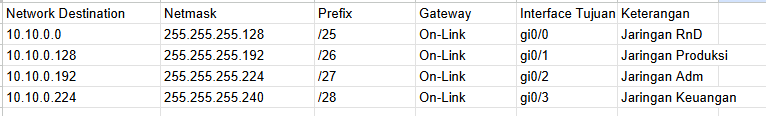
\includegraphics[width=0.5\linewidth]{Template Laporan Sementara/P1/Screenshot 2025-05-08 213508.png}
    \caption{Tabel No. 3}
    \label{fig:enter-label}
\end{figure}

